% This must be in the first 5 lines to tell arXiv to use pdfLaTeX, which is strongly recommended.
\pdfoutput=1
% In particular, the hyperref package requires pdfLaTeX in order to break URLs across lines.

\documentclass[11pt]{article}

% Style and Formatting for Camera-Ready PDF
\usepackage{naacl2021}

% Standard package includes
\usepackage{times}
\usepackage{latexsym}

% For proper rendering and hyphenation of words containing Latin characters (including in bib files)
\usepackage[T1]{fontenc}
% For Vietnamese characters
% \usepackage[T5]{fontenc}
% See https://www.latex-project.org/help/documentation/encguide.pdf for other character sets

% This assumes your files are encoded as UTF8
\usepackage[utf8]{inputenc}

% Defines how to include figures
\usepackage{graphicx}
\graphicspath{ {./Figures} }

% To rescale tables
\usepackage{adjustbox}

% For referencing the same footnote multiple times
%\makeatletter
%\newcommand\footnoteref[1]{\protected@xdef\@thefnmark{\ref{#1}}\@footnotemark}
%\makeatother

% This is not strictly necessary, and may be commented out,
% but it will improve the layout of the manuscript,
% and will typically save some space.
\usepackage{microtype}

% If the title and author information does not fit in the area allocated, uncomment the following
%
%\setlength\titlebox{<dim>}
%
% and set <dim> to something 5cm or larger.

\title{OTMISC: Our Topic Modeling Is Super Cool! \\ 
\large A Systematic Comparison of Topic Modeling Algorithms on Short and Long Text Datasets}

% Author information can be set in various styles:
% For several authors from the same institution:
% \author{Author 1 \and ... \and Author n \\
%         Address line \\ ... \\ Address line}
% if the names do not fit well on one line use
%         Author 1 \\ {\bf Author 2} \\ ... \\ {\bf Author n} \\
% For authors from different institutions:
% \author{Author 1 \\ Address line \\  ... \\ Address line
%         \And  ... \And
%         Author n \\ Address line \\ ... \\ Address line}
% To start a seperate ``row'' of authors use \AND, as in
% \author{Author 1 \\ Address line \\  ... \\ Address line
%         \AND
%         Author 2 \\ Address line \\ ... \\ Address line \And
%         Author 3 \\ Address line \\ ... \\ Address line}

%\author{First Author \\
%  Affiliation / Address line 1 \\
%  Affiliation / Address line 2 \\
%  Affiliation / Address line 3 \\
%  \texttt{email@domain} \\\And
%  Second Author \\
%  Affiliation / Address line 1 \\
%  Affiliation / Address line 2 \\
%  Affiliation / Address line 3 \\
%  \texttt{email@domain} \\}

\author{Berk Sudan \\
        Department of Informatics \\
        \texttt{berk.sudan@tum.de} \\\And
        Ferdinand Kapl \\
        Department of Mathematics \\
        \texttt{ferdinand.kapl@tum.de} \\\And
        Yuyin Lang \\
        Department of Informatics \\
        \texttt{yuyin.lang@tum.de}}

\begin{document}
\maketitle
\begin{abstract}
Topic modeling helps to classify documents into different topics and choose some words to represent the extracted topics. In this work, we created a topic modeling pipeline to evaluate different topic modeling algorithms, including their performance on short and long text, preprocessed and not preprocessed datasets, and with different embedding models (for embedding-based algorithms). Finally, we summarized the results and suggested how to choose algorithms based on the task. Our code is accessible on GitLab\footnote{\url{https://gitlab.lrz.de/practical-courses/nlp-lab-course-ss22/topic-modeling-advancements}}.

\end{abstract}
\section{Introduction}
Over the last few years, the availability of extensive unstructured data has risen to unseen heights. Especially text data, in the form of tweets, comments, news articles, customer reviews, and job postings, is everywhere, more than ever. This creates the need to be able to analyze these sizeable unstructured text datasets in order to derive insights from them. Topic Modeling is one of the domains that help humans understand these large corpora. Its goal is to cluster documents (in whatever form) into groups that share an underlying topic and then represent or associate these topics by a collection of so-called topic words that should be most descriptive of the topics at hand. The use-cases for Topic Modeling are manifold: online recommender systems trying to rank more relevant articles higher, extracting and mapping the right features of candidates to individual job postings, and last but not least, organizing extensive email collections, customer reviews as well as social media postings (see \citealp{lda-bert}). 

In general, Topic Modeling (in the following abbreviated as TM) algorithms can be divided into two categories: traditional probability-based approaches like Latent Dirichlet Allocation (LDA) (\citealp{lda}) or Non-negative Matrix Factorization (NMF) (\citealp{nmf}) and more modern embedding-based approaches like Top2Vec (\citealp{top2vec}), BERTopic (\citealp{bertopic}) or Cross-lingual Contextualized Topic Models (CTM) (\citealp{ctm}). These probability-based methods have some well-known shortcomings (see \citealp{lda-bert} and \citealp{bertopic}): for example, they need a predefined number of topics since they cannot dynamically create an estimate by "looking" at the dataset. Even more detrimental, they operate on bag-of-words inputs, disregard information encoded in the sequence of words, and, consequently, might lose semantic meaning. Newer algorithms try to solve these issues by employing pretrained embedding models. For example, BERTopic mainly uses embeddings from the Sentence-BERT framework (\citealp{sbert}) to encode the semantic information contained in the documents and then use the fact or assumption that vectors close in embedding space are semantically similar. Furthermore, hybrid approaches combine both worlds by concatenating LDA with embedding vectors, for example, LDA-BERT from \citet{lda-bert}. 

All available datasets are listed in Section~\ref{sec:datasets}, 
 and the algorithms are described in depth in Section~\ref{sec:algorithms}. The main goal of this work is to give a thorough overview of currently used, state-of-the-art TM algorithms and compare their performance on different short and long text datasets to suggest which approach should be favored for a given dataset.

\section{Related Work}
Currently, one of the biggest challenges in TM research is the lack of a golden standard for evaluating outputs from different algorithms. Even though all the existing methods work in different ways, all of them usually produce two things: An assignment of documents to topics/clusters\footnote{This can either be deterministic, as in one document belongs to one topic or probabilistic, i.e., there is a distribution over the topics for every document.} and a representation of every topic in the form of topic words with associated word scores that are metrics of the importance of that word for that topic.
%This lack of a standard will be illustrated by summarizing how some of the newer algorithms used here are evaluated in their respective paper. Then the result of a meta-analysis by \citet{incoherence} of forty different neural topic models and their current evaluation state will be presented. Finally, we propose our solution to this problem. 
In \citet{top2vec}, Top2Vec is only compared to the older methods of LDA and PLSA with the metric of \emph{Topic Information Gain} that tries to measure how informative topic words are in their respective documents. 
%Although this metric has an information-theoretic background, this paper is the only one that uses it, which makes comparisons with other results hard. Nevertheless, 
The outputs of the aforementioned three algorithms are compared on Yahoo Answers and 20 Newsgroups datasets. Finally, some non-metric findings are presented: Topics together with their respective topic words and visualizations of the semantic space by using UMAP to reduce the dimension of the embedding space to 2D and coloring the "points" by either real label\footnote{The labels were derived from 20 Newsgroups or Yahoo Answers.} or assigned topic. 

Before we continue, let us first introduce the most popular metrics for evaluating topic models: \emph{Topic Coherence} (abbreviated TC) and \emph{Topic Diversity} (TD). In this regard, various techniques exist for measuring the respective concepts. In general, coherence can be understood, as stated by \citet{incoherence}, as "An intangible sense, available to human readers, that a set of terms, when viewed together, enable human recognition of an identifiable category.". On the other hand, topic diversity is simply a measure of how diverse the topic words are, ranging from all topics described by the same words to all being different/unique. 

For example, in \citet{lda-bert}, LDA-BERT is compared to LDA, TF-IDF with K-Means, and BERT with K-Means by using $C_V$, a measure for topic coherence described in depth later, and silhouette score, a measure how well the clusters are separated, on a single dataset of Amazon product reviews. Furthermore, they only list the topic words of some resulting clusters for LDA-BERT. 
%it shows the visualizations of the clustering results, again by reducing their dimensions to 2D by UMAP, for all four mentioned methods but 

Finally, \citet{bertopic} sets an excellent example of how one can evaluate different algorithms. First, BERTopic is compared to LDA, NMF, Top2Vec, and CTM, thus including newer methods, on three different datasets composed of long text (20 Newsgroups, BBC News) and a short text dataset (Trump's tweets). Then, TC and TD measures are used, i.e., NPMI and percentage of unique topic words, but unfortunately, no visualizations or examples of topic words are given other than a graphic of the computation times of all algorithms. 

Our observations on this small subset of current methods are supported by the findings in \citet{incoherence}: There exists a \emph{validation gap} since automated coherence measures that were validated in the past on topics produced by classical TM algorithms are not validated yet on the outputs of current (neural) methods.
%In short, there is no guarantee that existing automated coherence measures are a reasonable estimate of the "real" coherence, as scored by humans, of topic words produced by neural algorithms. 
Furthermore, they also recognize a \emph{standardization gap}. This is because most works on TM do not use the same benchmarking data, preprocessing steps, and hyperparameter tuning procedures.
%For example, in their meta-analysis of forty recent neural TM papers, none of them used a human evaluation of coherence, a lot of them did not specify the exact measurements used for evaluating coherence,
%\footnote{For example, not specifying window size or reference corpus for NPMI.}
%over one-fifth did not use recent baselines,
%\footnote{A "good" example is Top2Vec, although it was not included in this meta-analysis.}
%and not all of them used multiple runs with averaging of results. 
To add, experiments by \citet{incoherence} show that human assessment of coherence differs from automatic measures, e.g., NPMI and $C_V$, in the sense that automatic scores declare a clear winner of the topic model when humans do not. They explain this difference by multiple factors: metric-based evaluation favors esoteric topics by producing high NPMI scores for topic words that are very specific and only occur in a narrow context, and by giving low scores to words that are related (for humans) but do not frequently appear in a small context window (NPMI: 10-word tokens). Therefore it makes sense to prefer $C_V$ over NPMI as a coherence measure as it uses a larger window size; details for that choice are given later. 
%Another reason for the discrepancy is that some topic words do not make sense together without an in-depth knowledge of the data, i.e., humans give a low score to topic words with a high metric score as they appear frequently in the documents analyzed. 
In general, there needs to be a reconsideration of how to evaluate topic models, both by humans and automatic metrics. Possible directions for further research are given in Section~\ref{sec:future}. 

Finally, our solution for evaluating topic models is an exhaustive combination of different topic coherence, diversity, and cluster metrics together with many visualizations which facilitate better comprehension and evaluation of the outputs of topic models by humans. The used metrics consist of the following: 
\begin{itemize}
\item \textbf{Normalized Pointwise Mutual Information:} NPMI is a measure for the coherence of topic words in [-1,1], with 1 being perfect association.

\item \textbf{C${_\mathbf{V}}$:} It is also a coherence measure but uses a larger sliding window (110-word tokens) over the text with indirect cosine similarity based on NPMI; in [0,1] with 1 being perfect association. This metric is motivated by the survey by \citet{coherence_survey} of "all" sensible combinations of existing and new coherence measures where it achieved the best results in terms of highest correlation with human judgment. 

\item \textbf{Topic Diversity:} A measurement for diversity as a percentage of unique topic words, i.e., in [0,1] with 1 meaning all different topic words. 

\item \textbf{Inverted Rank-Biased Overlap:} Also a measure for diversity as a rank-weighted percentage of unique topic words where words at higher ranks are penalized less. Again in the range of [0,1] with 1 meaning all different topic words. 

\item \textbf{Rand Index:} Similarity measure for the two clusterings given by the topic model and the real labels (details later in Section~\ref{sec:datasets}), again in [0,1] with 1 representing a perfect match. 
\end{itemize}

The first four, so all topic coherence and diversity metrics are implemented using the framework OCTIS\footnote{\url{https://github.com/MIND-Lab/OCTIS}}, an open-source python package (\citealp{octis}), and the rand index from scikit-learn.\footnote{\url{https://scikit-learn.org/stable/modules/generated/sklearn.metrics.rand_score.html}}

Additionally, depending on the algorithm, as many as five different visualizations are available for the output of a topic model. Details are given in Section~\ref{sec:design}. 

At the end of this section, we briefly mention other works comparing recent topic models. For example, in \citet{tm_comparison}, four TM algorithms are compared on a dataset of tweets consisting of covid travel-related hashtags. Namely, they compare the performance of LDA, NMF, Top2Vec, and BERTopic by topic coherence of the best scoring model for the respective algorithm. 
%Therefore the number of topics, either specified or determined by the algorithm, differs for all of them. Their experiments include a manual inspection of the topic words per topic and an interpretation from a social science point of view. Moreover, 
The following approach is suggested for determining the number of topics for a given dataset. First, choosing an \emph{optimal} number is hard or even impossible because topics frequently overlap, and topics are often mixtures of background "themes". Nevertheless, they recommend choosing a small number to allow for manual (human) inspection of the resulting topics, for example, 10, and then going from there. Finally, their conclusion determines BERTopic as a winner on this short text dataset and lists the strengths as well as weaknesses of the respective algorithms. As far as we know, this work is one of the only ones comparing current TM models with older baselines, other than works on new algorithms such as \citet{bertopic}. Another relevant work for our experiments is \citet{lda-bert_survey}. Many combinations of LDA, Word2Vec, Doc2Vec, and BERT with dimension reduction methods (PCA, t-SNE, Autoencoder) and the clustering algorithm K-Means were compared on the 20 Newsgroups by using Normalized Mutual Information as an evaluation metric. The best performing composition was what we call LDA-BERT, a hybrid approach of LDA together with Sentence BERT followed by an Autoencoder and K-Means. However, they only evaluated LDA-BERT on a subset of one-fourth of the whole dataset due to, as they write, computation time constraints.

\section{Architectural Design}
\label{sec:design}

Now we want to describe the architecture of our pipeline for running the experiments, whose results are shown later in Section~\ref{sec:comparison}. The name of our framework is an homage to OCTIS, and we called it OTMISC: Our Topic Modeling Is Super Cool! and as can be seen in appendix \ref{sec:app_architecture} in figure \ref{fig:architecture}, our framework currently contains eight different datasets, described in Section \ref{sec:datasets}, sixteen preprocessing methods, six TM algorithms and for evaluation five visualizations as well as the five already mentioned automatic metrics. The list of available preprocessing functions can be seen in Appendix \ref{sec:pre_func} in Table \ref{tab:pre_func_non_tok} (applied to raw text) and Table \ref{tab:pre_func_tok} (applied to tokenized text). Furthermore, the available visualizations consist of:

\begin{itemize}
\item \textbf{UMAP 2D Scatter Plot:} Visualizes document embeddings colored by their topic cluster.
\item \textbf{Topic Words Bar Chart:} Plots the top words of every topic with their word scores.
\item \textbf{Labels per Topic:} Shows the distribution of real labels of documents (see Section \ref{sec:datasets}) per topic cluster.
\item \textbf{Topic Similarity Matrix:} Matrix colored by cosine similarity between topic embeddings for similarity of topics in embedding space.
\item \textbf{Representative Documents:} Colored dataframe with representative documents per topic. 
\end{itemize}

The UMAP 2D scatter plot and topic similarity matrix visualization are only available for Top2Vec, BERTopic, and LDA-BERT. Example outputs will be shown later.

\section{Datasets}
\label{sec:datasets}
 
The datasets used here can be divided into two different categories: short and long text datasets. Dividing them into these categories is justified because a dataset with short text has inherently different characteristics than an extended text dataset. For example, tweets from \emph{CRISIS \#01} (short for CRISIS NLP - Resource \#01) often contain fewer than 30 words and many URLs, hashtags, and typos or abbreviations. In contrast, long text datasets like 20 Newsgroups often have documents with more than 100 words and are more readable and more sophisticated as they are often news articles. All datasets, their categories, number of documents, and number of real labels as given by the sources are shown in Table \ref{tab:datasets}. Their respective sources can be accessed in the footnotes. For example, the 20 Newsgroups dataset is the by-date version\footnote{\url{http://qwone.com/~jason/20Newsgroups}}, Yahoo Answers is a subset of 60k documents from the full dataset\footnote{\url{https://github.com/LC-John/Yahoo-Answers-Topic-Classification-Dataset}}, the CRISIS NLP - Resources are only the labeled versions\footnote{\label{foot:crisis}\url{https://crisisnlp.qcri.org/}}, and the AG News Titles are the title of various news\footnote{\url{https://huggingface.co/datasets/ag_news}}. Note that, due to its size, the dataset "AG News Titles + Text" , which is a concatenation of news titles and their contents, is ignored in the initial experiments.

\begin{table}[ht]
\centering
\begin{adjustbox}{width=0.5\textwidth}
\begin{tabular}{lccc}
\hline
\textbf{Name} & \textbf{Type of Text} & \textbf{\# Docs} & \textbf{Topic Count} \\
\hline
20 Newsgroups (By Date) & Long & 18846 & 20\\ 
Yahoo Answers (60K) & Long & 60000 & 10\\
AG News Titles + Text & Long & 127600 & 4\\
CRISIS \#01 & Short & 20514 & 4\\
CRISIS \#07 & Short & 10941 & 2\\
CRISIS \#12 & Short & 8007 & 4\\
CRISIS \#17 & Short & 76484 & 10\\
AG News Titles & Short & 127600 & 4\\
\hline
\end{tabular}
\end{adjustbox}
\caption{ Available datasets and their characteristics}
\label{tab:datasets}
\end{table}

For our experiments, we initially explored how unprocessed and preprocessed versions of the same dataset affect the results. Even for embedding-based TM algorithms such as Top2Vec and BERTopic, we observed that a small amount of preprocessing (removal of stop-words and non-informative words) resulted in better topic words. Therefore, to compare different algorithms/datasets fairly, we used similar preprocessing methods in each run. 
%The preferred methods are "to\_lowercase", "standardize\_accented\_chars", "remove\_url", "expand\_contractions", "remove\_mentions", "remove\_hashtags", "keep\_only\_alphabet", "remove\_english\_stop\_words" and "lemmatize\_noun". Note that this is just a subset of our tool's available (currently 16) preprocessing methods.

Moreover, to enable an easier human-based comparison and good visualizations of the outputs, we chose a low number of topics per dataset as given by the number of unique labels in the respective datasets (see Table \ref{tab:datasets}).

\section{Algorithms}
\label{sec:algorithms}

In this section, we introduce six algorithms in our tool in more detail. Here, we present how the algorithms work, what parameters we use, and provide visualization examples for the algorithms.

\subsection{LDA and NMF}
First, we introduce LDA and NMF together. As the only probability-based approaches in this work, they have in common that they both use the BOW (Bag of Words) model. More specifically, LDA iterates two probabilities -- P(topic t | document d) and P(word w | topic t) through words to obtain topic words and topic documents. On the other hand, NMF uses matrix factorization to convert a high-dimensional representation into the product of two low-dimensional representations to achieve the same goal.

We use OCTIS for the implementation. We set the parameter alpha for LDA as asymmetric; for NMF, we use the default settings in OCTIS. We predefine the topic numbers for both algorithms as the topic count in Table \ref{tab:datasets} and set a random state for them for reproducibility. We show the labels per topic visualization of NMF on Crisis 12 dataset in Appendix \ref{appendix_labels_per_topic_visualization}.

\subsection{BERTopic}
Next, we briefly describe how BERTopic creates topics and topic representations in the form of topic words. The algorithm can be split into three phases. In \emph{phase 1}, embeddings are created for each document in the data by leveraging a pretrained embedding model. By default, any model from the Sentence BERT framework is supported (\citealp{sbert}) but generally, which is one of the biggest strengths of BERTopic, any pretrained language model that was fine-tuned on semantic similarity can be used by passing it the calculated embeddings. Then in \emph{phase 2}, these embeddings are reduced in dimension by UMAP (\citealp{umap}), and then the lower-dimensional representations are clustered into topics by a hierarchical clustering algorithm with a soft-clustering approach HDBSCAN (\citealp{hdbscan}). This clustering method allows documents to be classified as noise which might improve the generation of concise topics. However, in practice, we found that when using a low number of topics\footnote{here, “low” means in comparison to the number of topics found by the algorithm before reducing it to a given number of topics}, a large portion of the files tends to be classified as noise, up to 60\% of the full dataset. Here each document is assigned to one topic (cluster), so if one wants to assign every document to a "real", non-noise cluster, our experiments showed that the most simple and elegant solution is to use K-Means instead of HDBSCAN, which of course requires us to specify the number of desired topics, also producing good results. Other options like changing the parameters of the HDBSCAN algorithm and assigning documents to the most likely non-noise cluster when the probability is more significant than a specified threshold came with additional problems and performance drops. Finally, in \emph{phase 3}, topic words per cluster are extracted by creating topic-word distributions with a class-based TF-IDF approach and taking the top n words with the highest probability (here: ten words per topic). A topic similarity matrix visualization example can be found in Appendix \ref{appendix_topic_similarity_matrix}.

\subsection{LDA-BERT}
As previously mentioned, LDA-BERT is a hybrid approach combining a classical TM algorithm with embeddings. First, for every document, LDA generates a vector with the probabilities of this document belonging to a topic, so if we choose several topics equal to 10, this vector has dimension 10 for every document. Then the LDA vector is concatenated with the embedding vector; we use an embedding model again from the Sentence BERT framework, using a hyperparameter gamma weighting the respective importance of the two vectors. Next, an autoencoder produces a latent space representation of this concatenated vector which is finally clustered using K-Means, and the topic words for each cluster are simply the most frequent words per cluster. Therefore this method and our implementation benefit highly from preprocessing.\footnote{Our implementation of LDA-BERT is an adaptation of the following notebook: \url{www.kaggle.com/code/dskswu/topic-modeling-bert-lda}}. Appendix \ref{appendix_draw_representative_documents} illustrates how representative documents of the detected topics look like after running LDA-BERT.

\subsection{Top2Vec}
There are several similarities between Top2Vec and BERTopic. They both use pretrained embedding models to create document and word embeddings. Embedding dimensions are then reduced by UMAP and clustered by HDBSCAN. Unlike BERTopic, Top2Vec adopts a slightly different approach to generating topic words, assigning all documents to a topic. Therefore, Top2Vec outputs do not contain \emph{noisy} documents which are not assigned to a topic. Moreover, Top2Vec deals with the outlier documents problem by simply not taking them into account while computing topic vectors, although still assigning them to the closest topic vectors afterward. Outlier documents can be observed by the naked eye, thanks to the UMAP-2D visualization method. An example UMAP-2D output can be found in Appendix \ref{appendix_umap2d_visualization}. In addition, \citet{top2vec} concludes that Top2Vec consistently finds more informative topics and representative of the corpus than probabilistic generative models like LDA and PLSA for varying sizes of topics and number of top topic words. We strongly agree with this conclusion since we also noticed a similar pattern in our experiments.

We used the library from the original author of the Top2Vec paper with some adjustments and improvements\footnote{\url{https://github.com/ddangelov/Top2Vec}}. It was suggested that some preprocessing methods, namely stop-words removal and lemmatization, are noneffective as creating word embeddings can overcome these issues (\citealp{top2vec}). However, after applying the aforementioned preprocessing methods, we observed minor improvements in the results, especially for short text tweet datasets. We reduced the number of detected topics to the number of real topics using \emph{hierarchical topic reduction}. Top2Vec and BERTopic do not need the number of topics to be provided in advance, although we did to make a fair comparison according to the evaluation metrics. It also helped us to see whether each detected topic could be matched with a different real label. We argue that the main disadvantage of hierarchical topic reduction is the requirement of a \emph{balance} in the number of documents per topic because there is a higher chance for the topics of similar sizes to merge. If the dataset is highly unbalanced, this can lead to the merging of unrelated documents.

\subsection{CTM}
As the newest algorithm in our task, Contextualized Topic Models (CTM) also uses embedding models. This algorithm is based on variational autoencoders. Instead of inputting BOW, CTM uses pretrained multilingual representations from SBERT, thus taking the context information into account. In this way, CTM overcomes the biggest drawback of BOW representation: BOW has no information about the context.

We use OCTIS for the implementation of CTM. In this work, we tried three different embedding models for CTM (“bert-base-nli-mean-tokens”, “all-MiniLM-L6-v2”, “paraphrase-multilingual-MiniLM-L12-v2”). Since CTM computations take much time, we did not use preprocessing to save time. In Appendix \ref{appendix_top_words_bar_chart}, we present the topic words bar chart visualization to show its performance.

\section{Comparison}
\label{sec:comparison}
In this section, we report and compare the results of our algorithms, including performance results on short and long datasets, performance results on preprocessed and unprocessed datasets, and impacts of different embedding models. We further discuss the result in Section \ref{sec:discussion}.

\subsection{Performance on Short Datasets}
First, we compare the performance of different algorithms on short datasets. As stated before, short datasets in our task include four crisis datasets and one news dataset (AG News Titles). Table \ref{tab:short datasets} shows the results of our algorithms on all five evaluation metrics. The scores are averaged over all five datasets. The best-performing algorithm is marked in bold. Moreover, the number in the parenthesis indicates the ranking of each algorithm.

\begin{table}[ht]
\centering
\begin{adjustbox}{width=0.5\textwidth}
\begin{tabular}{lccccc}
%\begin{tabular}{@{\extracolsep{5pt}}lcc}
\hline
\textbf{} & \textbf{TD} & \textbf{TD} & \textbf{TC} & \textbf{TC} & \textbf{Cluster}\\
\textbf{Algorithm} & \textbf{Unique} & \textbf{Inv. RBO} & \textbf{NPMI} & \textbf{C${_\mathbf{V}}$} & \textbf{Rand}\\
\hline
NMF & 0.718(5) & 0.715(6) & -0.014(4) & 0.388(5) & 0.614(5)\\ 
LDA & 0.700(6) & 0.810(4) & 0.010(2) & 0.435(3) & 0.625(4)\\
LDA-BERT & 0.743(4) & 0.778(5) & -0.001(3) & 0.421(4) & 0.727(3)\\
BERTopic & 0.826(3) & 0.901(3) & \textbf{0.050(1)} & \textbf{0.493(1)} & 0.474(6)\\
Top2Vec & 0.897(2) & 0.956(2) & -0.279(6) & 0.388(5) & 0.739(2)\\
CTM & \textbf{0.966(1)} & \textbf{0.994(1)} & -0.100(5) & 0.486(2) & \textbf{0.746(1)}\\
\hline
\end{tabular}
\end{adjustbox}
\caption{Performance on short datasets}
\label{tab:short datasets}
\end{table}

As Table \ref{tab:short datasets} suggests, CTM outperforms other algorithms in TD and Cluster Rand, while BERTopic achieves the best score in TC. It is also interesting to note that CTM obtains a good result in TC (C${_\mathbf{V}}$), and the gap with BERTopic is not much.

\subsection{Performance on Long Datasets}
The comparison on long datasets is quite similar to the short ones. For example, we have the 20 Newsgroups dataset and Yahoo Answers dataset; the result is the average score of these two datasets. The number in the parenthesis indicates the ranking of each algorithm. The result is shown in Table \ref{tab:long datasets}.

\begin{table}[ht]
\centering
\begin{adjustbox}{width=0.5\textwidth}
\begin{tabular}{lccccc}
\hline
\textbf{} & \textbf{TD} & \textbf{TD} & \textbf{TC} & \textbf{TC} & \textbf{Cluster}\\
\textbf{Algorithm} & \textbf{Unique} & \textbf{Inv. RBO} & \textbf{NPMI} & \textbf{C${_\mathbf{V}}$} & \textbf{Rand}\\
\hline
NMF & 0.565(3) & 0.805(5) & 0.035(4) & 0.508(4) & 0.846(4)\\ 
LDA & 0.525(5) & 0.878(3) & 0.038(3) & 0.538(3) & 0.792(5)\\
LDA-BERT & 0.397(6) & 0.661(6) & 0.055(2) & \textbf{0.594(1)} & 0.880(2)\\
BERTopic & 0.637(2) & 0.828(4) & \textbf{0.081(1)} & 0.577(2) & 0.425(6)\\
Top2Vec & \textbf{0.819(1)} & 0.902(2) & -0.113(6) & 0.436(5) & \textbf{0.906(1)}\\
CTM & 0.552(4) & \textbf{0.909(1)} & -0.056(5) & 0.404(6) & 0.861(3)\\
\hline
\end{tabular}
\end{adjustbox}
\caption{Performance on long datasets}
\label{tab:long datasets}
\end{table}

The situation for long datasets is much more complicated than for short datasets. A total of four algorithms received first place in at least one evaluation metric. Top2Vec wins first place twice: In TD (Unique) and Cluster Rand; it also wins second place in TD (Inv. RBO) with a small gap to first place. As for the two metrics in TC, LDA-BERT and BERTopic each receive first and second place, outperforming other algorithms.

\subsection{Performance on Preprocessed and Unprocessed Datasets}
The preprocessing of datasets strongly influences the performance of the algorithms. For LDA and NMF, because of the BOW representation, preprocessing is essential. Otherwise, the model assigns immense importance to those words which appear quite often in all documents, including stop words and hashtags. Even for embedding-based methods in our work, if we do not apply preprocessing methods, the extracted topic words would contain too many stop words. Therefore, it is interesting to see how preprocessing influences performance based on various evaluation metrics. Here, we choose one probability-based algorithm (NMF) and one embedding-based algorithm (BERTopic). To keep the table not too big, we present the performance on 20 Newsgroups dataset (a long dataset) and CRISIS \#01 (a short dataset) on the five evaluation metrics. The result is shown in Table \ref{tab:pre and not pre datasets nmf} and Table \ref{tab:pre and not pre datasets BERTopic}. "pre" in the parenthesis means the result is obtained on the preprocessed dataset.

\begin{table}[ht]
\centering
\begin{adjustbox}{width=0.5\textwidth}
\begin{tabular}{lccccc}
\hline
\textbf{} & \textbf{TD} & \textbf{TD} & \textbf{TC} & \textbf{TC} & \textbf{Cluster}\\
\textbf{Dataset} & \textbf{Unique} & \textbf{Inv. RBO} & \textbf{NPMI} & \textbf{C${_\mathbf{V}}$} & \textbf{Rand}\\
\hline
20 Newsgroups (pre) & 0.640 & 0.960 & 0.103 & 0.646 & 0.736\\ 
20 Newsgroups & 0.370 & 0.822 & 0.023 & 0.470 & 0.836\\
\hline
Crisis \#01 (pre) & 0.825 & 0.878 & 0.089 & 0.492 & 0.522\\
Crisis \#01 & 0.600 & 0.740 & -0.008 & 0.388 & 0.586\\
\hline
\end{tabular}
\end{adjustbox}
\caption{Performance on preprocessed and not preprocessed datasets (NMF)}
\label{tab:pre and not pre datasets nmf}
\end{table}

\begin{table}[ht]
\centering
\begin{adjustbox}{width=0.5\textwidth}
\begin{tabular}{lccccc}
\hline
\textbf{} & \textbf{TD} & \textbf{TD} & \textbf{TC} & \textbf{TC} & \textbf{Cluster}\\
\textbf{Dataset} & \textbf{Unique} & \textbf{Inv. RBO} & \textbf{NPMI} & \textbf{C${_\mathbf{V}}$} & \textbf{Rand}\\
\hline
20 Newsgroups (pre) & 0.837 & 0.981 & 0.173 & 0.778 & 0.630\\ 
20 Newsgroups & 0.430 & 0.670 & 0.017 & 0.513 & 0.508\\
\hline
Crisis \#01 (pre) & 0.900 & 0.929 & 0.135 & 0.582 & 0.473\\
Crisis \#01 & 0.742 & 0.846 & -0.090 & 0.334 & 0.506\\
\hline
\end{tabular}
\end{adjustbox}
\caption{Performance on preprocessed and not preprocessed datasets (BERTopic)}
\label{tab:pre and not pre datasets BERTopic}
\end{table}

The scores in almost all the evaluation metrics have greatly improved. Only the score for Cluster Rand with NMF has dropped. The most significant gap appears in TD (Diversity) on 20 Newsgroups with BERTopic, which amounts to 0.397.

\subsection{Performance of Embedding-based Algorithm using Different Embedding Models}
Different embedding models vary in many aspects, such as embedding dimension, model size, data on which the model is pretrained, and so forth. In this work, we want to see whether the models perform differently when using different embedding models. In Table \ref{tab:datasets embeddings}, we present the performance of Top2Vec on four different embedding models and evaluate it on our five evaluation metrics. The number in the parenthesis indicates the ranking of each algorithm.

\begin{table}[ht]
\centering
\begin{adjustbox}{width=0.5\textwidth}
\begin{tabular}{lccccc}
\hline
\textbf{} & \textbf{TD} & \textbf{TD} & \textbf{TC} & \textbf{TC} & \textbf{Cluster}\\
\textbf{Embedding model} & \textbf{Unique} & \textbf{Inv. RBO} & \textbf{NPMI} & \textbf{C${_\mathbf{V}}$} & \textbf{Rand}\\
\hline
all-MiniLM-L6-v2 & 0.907(3) & 0.957(2) & -0.284(4) & 0.388(2) & \textbf{0.864(1)}\\ 
doc2vec & 0.912(2) & 0.931(4) & -0.276(3) & \textbf{0.485(1)} & 0.552(4)\\
paraphrase-multilingual & {} & {} & {} & {} & {}\\
-MiniLM-L12-v2 & \textbf{0.930(1)} & \textbf{0.987(1)} & \textbf{-0.252(1)} & 0.376(3) & 0.777(3)\\
universal-sentence-encoder & 0.860(4) & 0.941(3) & -0.267(2) & 0.366(4) & 0.827(2)\\
\hline
\end{tabular}
\end{adjustbox}
\caption{Performance with different embedding models}
\label{tab:datasets embeddings}
\end{table}

As the biggest embedding model in our work, “paraphrase-multilingual-MiniLM-L12-v2” received first place three times in the evaluation, including both TD evaluations. In TC, it performs similarly with doc2vec as both embedding models received first and third place. Finally, the embedding model “all-MiniLM-L6-v2” performs the best in Cluster Rand.

\section{Discussion}
\label{sec:discussion}
In this section, we discuss the results shown in Section \ref{sec:comparison}. Then, we draw conclusions based on our experiments and provide insight into TM.

\subsection{Can we suggest a golden algorithm for TM?}
As can be seen in Table \ref{tab:short datasets} and Table  \ref{tab:long datasets}, no algorithm outperforms others in all five evaluation metrics. This applies to both short and long datasets. Therefore, it is impossible to claim which algorithm is the best for TM. However, this does not mean we cannot give some suggestions about choosing proper algorithms because the choice of algorithms heavily depends on the specific task. For example, in some tasks, we expect the topic words to be more diverse; in others, we expect the coherence of topic words to be higher. Hence, it makes sense to suggest an algorithm that serves the purpose better for the given task.

For short datasets, CTM would be the first choice when TD and Cluster Rand are crucial for the task; but BERTopic should be considered first when we want to obtain a high TC score. Moreover, as the time complexity of CTM is high, Top2Vec is also a good choice if the computation resources are limited and achieving high TD/Cluster scores is the primary goal.

For long datasets, we encourage to use Top2Vec when it comes to TD. That is because compared to CTM, Top2Vec received a slightly lower score than CTM on TD (Inv. RBO), ranking second, but a much higher score on TD (Unique). Also, the high ranking in Cluster Rand made Top2Vec more comprehensive on long datasets. On the other hand, in the TC metric,  we recommend both LDA-BERT and BERTopic as their performances are similar. Furthermore, we noticed that in the four embedding-based algorithms, if one algorithm performs exceptionally well in TC or TD, it is likely to perform poorly in another evaluation metric, which should be considered when choosing the algorithm.

\subsection{Should we use preprocessed data?}
Data preprocessing should not be avoided for probability-based algorithms like LDA and NMF because such algorithms otherwise cannot read the context. Therefore, a considerable boost in performance is expected when using these algorithms. However, it is surprising that such a boost can also be seen when feeding preprocessed datasets to embedding-based algorithms such as BERTopic. Why does that happen? We argue that although embedding models help better understand the documents (this can be seen in Table \ref{tab:short datasets} and Table  \ref{tab:long datasets} as embedding-based algorithms perform much better than probability-based ones), they have no information about which words are representative. That is to say, just like probability-based algorithms, embedding-based algorithms assign high scores to stop words. Therefore, the strength of embedding models lies in obtaining the association between the topic words. Therefore, we strongly recommend using preprocessing methods when doing TM tasks.

\subsection{Does it make much difference to use different embedding models?}
Usually, the bigger the model size is, the more information a model can extract. However, a bigger model size does not necessarily produce a higher score. Moreover, it can be seen that in the three evaluation metrics where “paraphrase-multilingual-MiniLM-L12-v2” wins the first place, its score was not much higher than the last place. Therefore, embedding models do not influence much to the result, but only slightly.

One should also remember that bigger models will lead to longer computation time. In our work, “all-MiniLM-L6-v2” and “doc2vec” are much faster to compute. Since their performances are not bad, it is worth considering them if the computation resources are limited.

\section{Future Work}
\label{sec:future}

Two areas of TM that need to be improved the most are topic representations and evaluation of them or topic models in general. The current state of topic representations is using topic words, and as already highlighted in \citet{incoherence}, there is a need for something better. Humans usually describe a topic with a short paragraph, often including examples, so a simple list of (topic) words is just not enough to comprehend a topic in a collection of documents. Furthermore, the evaluation of topic models is in dire need of new metrics or improved human-based scoring to better compare existing and upcoming algorithms, especially for neural, non-classical methods. 

One of the most exciting avenues of further research is the composition of already used methods. Many newer approaches consist of the following building blocks: a pretrained language model for the embedding, a dimension reduction, and clustering algorithm, and a method to extract topic representations of the existing clusters. For example, further experiments on LDA-BERT are of interest: combining different representations of documents, embeddings, or probabilistic vectors, with newer dimensions and clustering solutions (UMAP \& HDBSCAN) with improved topic word representations (class-based TF-IDF). Similar experiments for newly developed dimension reduction and cluster algorithms are imaginable, including building full pipelines to fine-tune a given dataset. 

Finally, we would like to look more into the noise clusters BERTopic produces: Are they helpful by letting the existing topics be more concise and descriptive, or are they just an obstacle in understanding a collection of documents?

\section{Conclusion}
\label{sec:conclusion}
TM has been more and more applied in our daily life, and the need to extract topics from unstructured data is also increasing daily. In our work, we created a pipeline for TM, including choosing datasets, algorithms, and evaluation metrics. Apart from that, we also realized five visualization methods to help humans evaluate the model performance intuitively.

In our experiments, we found that no algorithm beats others in all the evaluation metrics; thus, a golden algorithm does not exist. However, one can choose the best algorithm according to the task. Moreover, even though embedding-based models perform better than probability-based ones, using preprocessed data as input is still beneficial. Finally, different embedding models can bring some performance differences, but not much. Here, the longer computation time caused by a bigger embedding model should be considered.

%We hope our work can facilitate the use of TM models and make them more and more popular.

\nocite{*}

\section*{Acknowledgements}
We want to thank Miriam Anschütz and Ahmed Mosharafa for their assistance and valuable feedback at every project stage.

% Includes only your custom bibliography per default. See above for how to include anthology files.
\bibliography{custom_tm}
\bibliographystyle{acl_natbib}

\newpage

\appendix

\section{Appendix - Architectural Design}
\label{sec:app_architecture}

\begin{figure}[ht]
%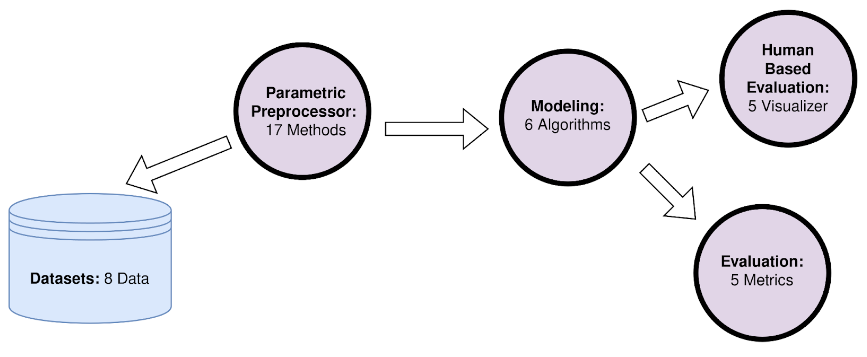
\includegraphics[width=8cm]{Figures/architecture_horizontal.png}
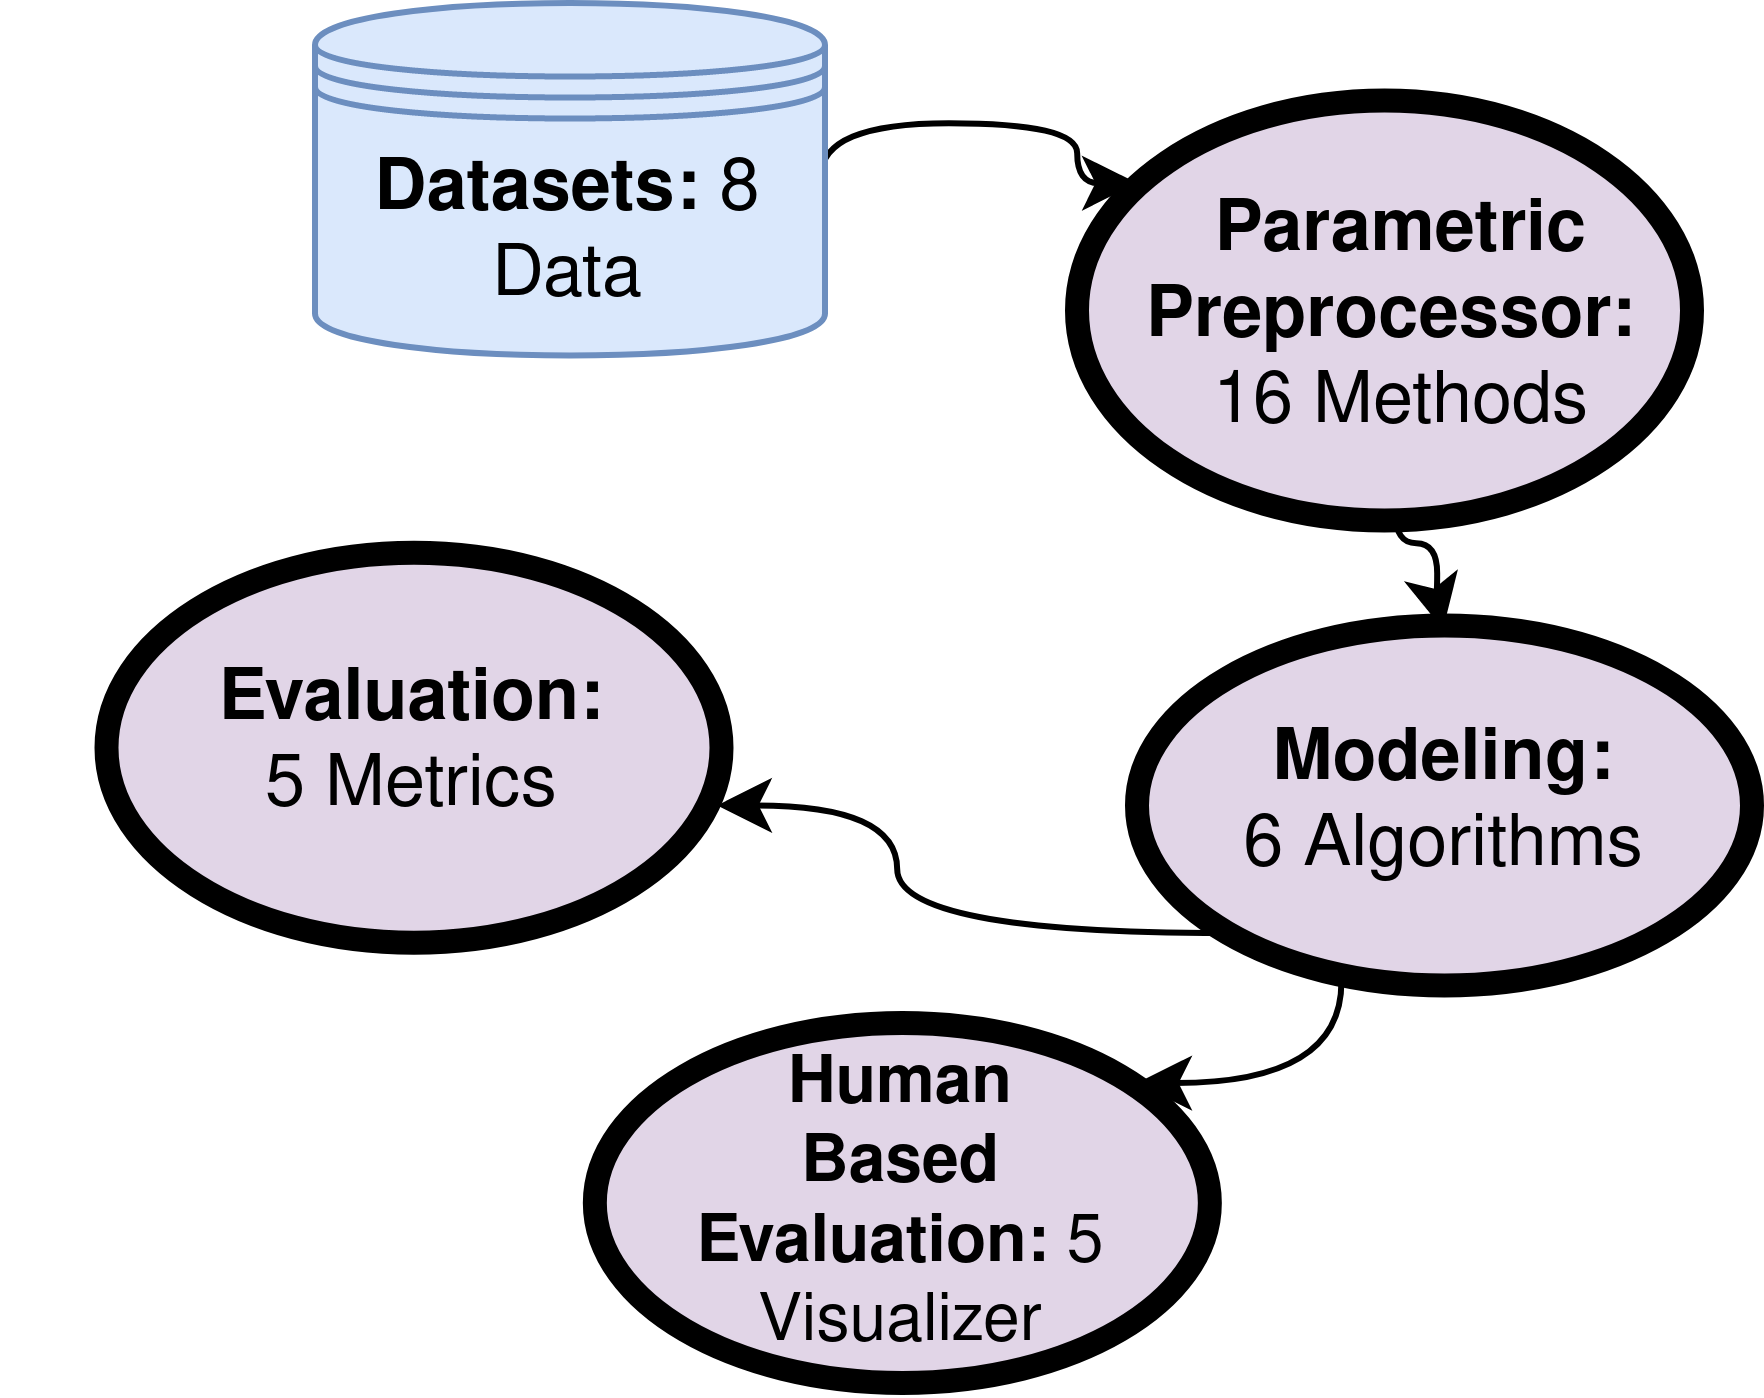
\includegraphics[width=5.5cm]{Figures/architecture_vertical.png}
\centering
\caption{Architectural Design of OTMISC Pipeline}
\label{fig:architecture}
\end{figure}

\section{Appendix - Visualizations}
\label{sec:appendix}
In this section, we present five different visualization methods with examples.
\subsection{Labels Per Topic Visualization} \label{appendix_labels_per_topic_visualization}
This visualization (Figure \ref{fig:labels per topic}) shows the performance of NMF in grouping the documents that belong to the same real label into the same detected topic. For example, in topic 1, most of the documents assigned to this topic have the real label \emph{earthquake}. We conclude that the model performs better when different real labels dominate each detected topic. As it can be seen, the distinction here is primarily obvious, while there are some \emph{mixed} topics, such as topic 2.

\subsection{Topic Similarity Matrix}\label{appendix_topic_similarity_matrix}
Figure \ref{fig:topic_similarity_matrix} shows the topic similarity matrix for BERTopic with 20 Newsgroups. Only five topics are shown here as a subset of 20 to avoid too big a figure. The numbers in the matrix indicate the cosine similarity of different topics. Low values indicate that the two topics are irrelevant, while high values suggest the opposite. For example, topic five and topic twelve can be considered similar topics in politics.

\subsection{Top Topic Words Bar Chart}\label{appendix_top_words_bar_chart}
This visualization (Figure \ref{fig:topic words}) shows the performance of CTM on CRISIS \#12 about the topic words. It is clear in the figure that the topic words belong to four different topics: Wildfire, cyclone, flood, and earthquake.

\subsection{UMAP 2D Scatter Plot}\label{appendix_umap2d_visualization}

A UMAP-2D visualization output can be seen in Figure \ref{fig:umap2d} for Top2Vec with the dataset Crisis \#12. The outlier documents are marked with white circles, and each color represents a different detected topic (not real label). Since it directly uses document embeddings, this visualization method is only available for embedding-based algorithms (Top2Vec, BERTopic, and LDA-BERT). Leveraging the UMAP algorithm reduces the number of document dimensions to 2 and visualizes the resulting vectors in a 2D coordinate system.

\subsection{Representative Documents} \label{appendix_draw_representative_documents}
Figure \ref{fig:representative_docs} shows the performance of LDA-BERT on the CRISIS \#12 dataset. It is convenient to see the sentences (or documents) that obtain the highest scores; thus, this visualization is crucial for human-based evaluation. 

\section{Appendix - Preprocessing Functions}
\label{sec:pre_func}
Here, we show the preprocessing functions used in our work. Table \ref{tab:pre_func_non_tok} shows the functions for raw texts. These functions could be used on the entire sentence. Table \ref{tab:pre_func_tok} shows the functions for tokenized texts, which means these functions are specific for words, for example, deleting or changing the form of a word.

The preferred methods in our work are "to\_lowercase", "standardize\_accented\_chars", "remove\_url", "expand\_contractions", "remove\_mentions", "remove\_hashtags", "keep\_only\_alphabet", "remove\_english\_stop\_words" and "lemmatize\_noun".

\begin{table}[ht]
\centering
\begin{adjustbox}{width=0.5\textwidth}
\begin{tabular}{p{0.25\textwidth}p{0.25\textwidth}}
\hline
\textbf{Function} & \textbf{Description}\\
\hline
to\_lowercase &  text to lowercase \\ 
standardize\_accented\_chars & standard representation\newline for accented characters \\
remove\_url & remove www and http(s) links \\ 
expand\_missing\_delimiter & insert space between a lower- and uppercase letter \\ 
remove\_mentions & remove @user \\
remove\_hashtags & remove \#hashtag  \\ 
keep\_only\_alphabet & keep only letters from a-z \\
remove\_new\_lines & remove newline characters \\
remove\_extra\_spaces & delete additional spaces \\
remove\_html\_tags & remove all <...> tags \\\hline
\end{tabular}
\end{adjustbox}
\caption{Available preprocessing functions applicable to non-tokenized text}
\label{tab:pre_func_non_tok}
\end{table}

\begin{table}[ht]
\centering
\begin{adjustbox}{width=0.5\textwidth}
\begin{tabular}{p{0.25\textwidth}p{0.25\textwidth}}
\hline
\textbf{Function} & \textbf{Description}\\
\hline
expand\_contractions & example: do not, I will, ... \\ 
remove\_english\_stop\_words & example: I, is, and, ... \\ 
lemmatize\_noun,\newline lemmatize\_verb,\newline lemmatize\_adjective & lemmatize words with respective part of speech tag \\ 
correct\_typo & substitutes words with detected typo correction \\
\hline
\end{tabular}
\end{adjustbox}
\caption{Available preprocessing functions applicable to tokenized text}
\label{tab:pre_func_tok}
\end{table}

\begin{figure*}[ht]
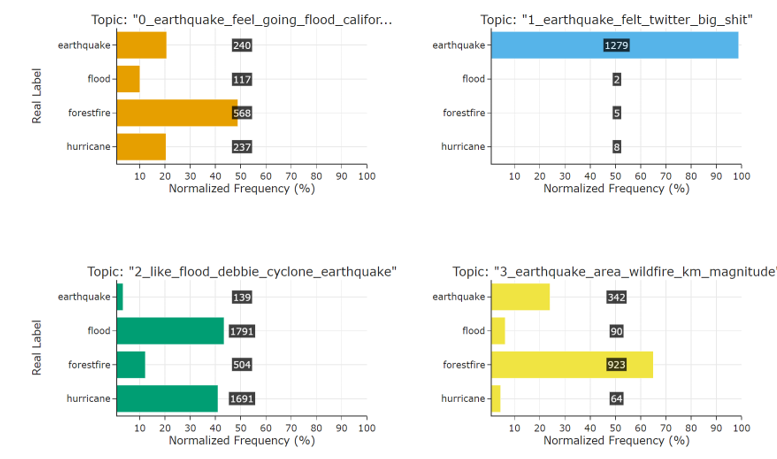
\includegraphics[width=16cm]{Figures/labels_per_topic.png}
\centering
\caption{Labels per Topic Visualization for NMF}
\label{fig:labels per topic}
\end{figure*}

\begin{figure*}[ht]
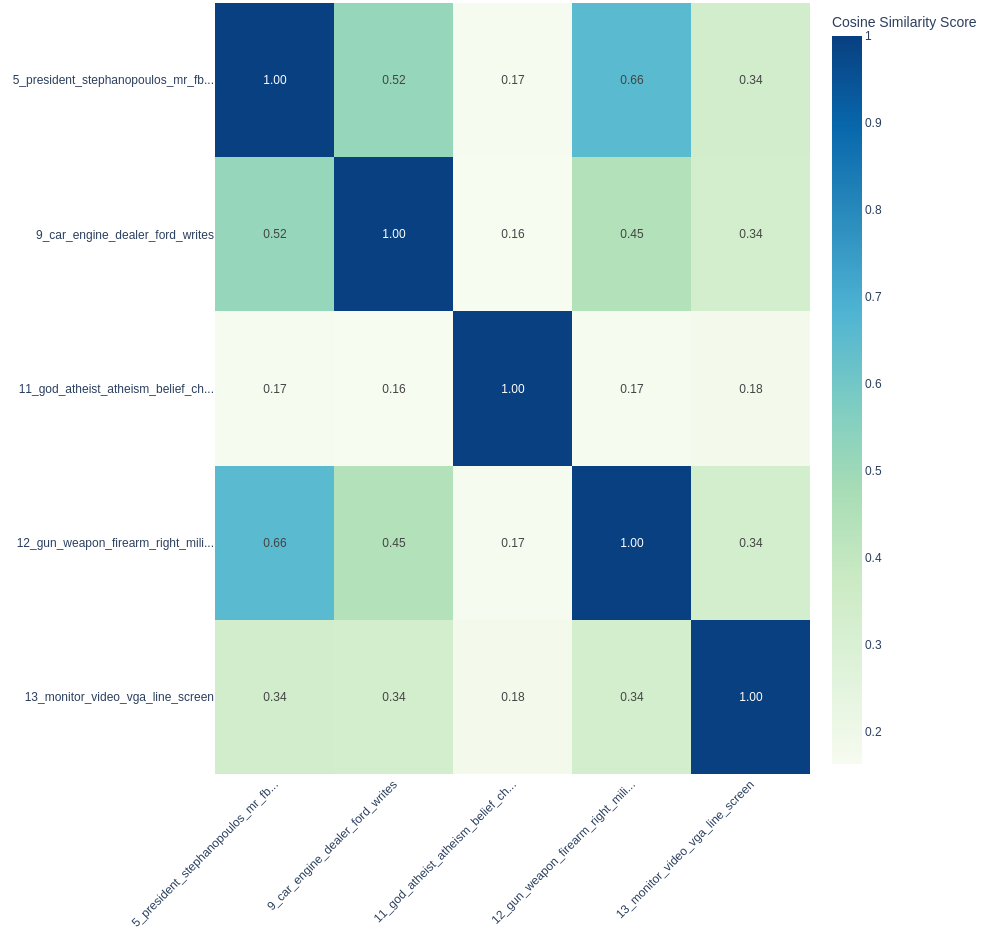
\includegraphics[width=17cm]{Figures/bertopic_topic_sim_matrix_20news}
\centering
\caption{Topic Similarity Matrix Visualization for BERTopic}
\label{fig:topic_similarity_matrix}
\end{figure*}


\begin{figure*}[ht]
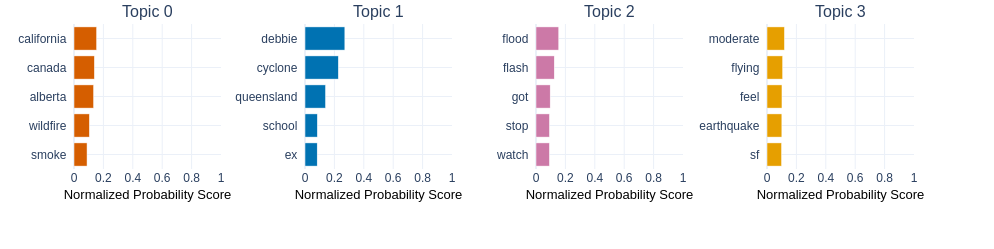
\includegraphics[width=14cm]{Figures/ctm_topic_words_crisis_12.png}
\centering
\caption{Top Topic Words Visualization for CTM}
\label{fig:topic words}
\end{figure*}

\begin{figure*}[ht]
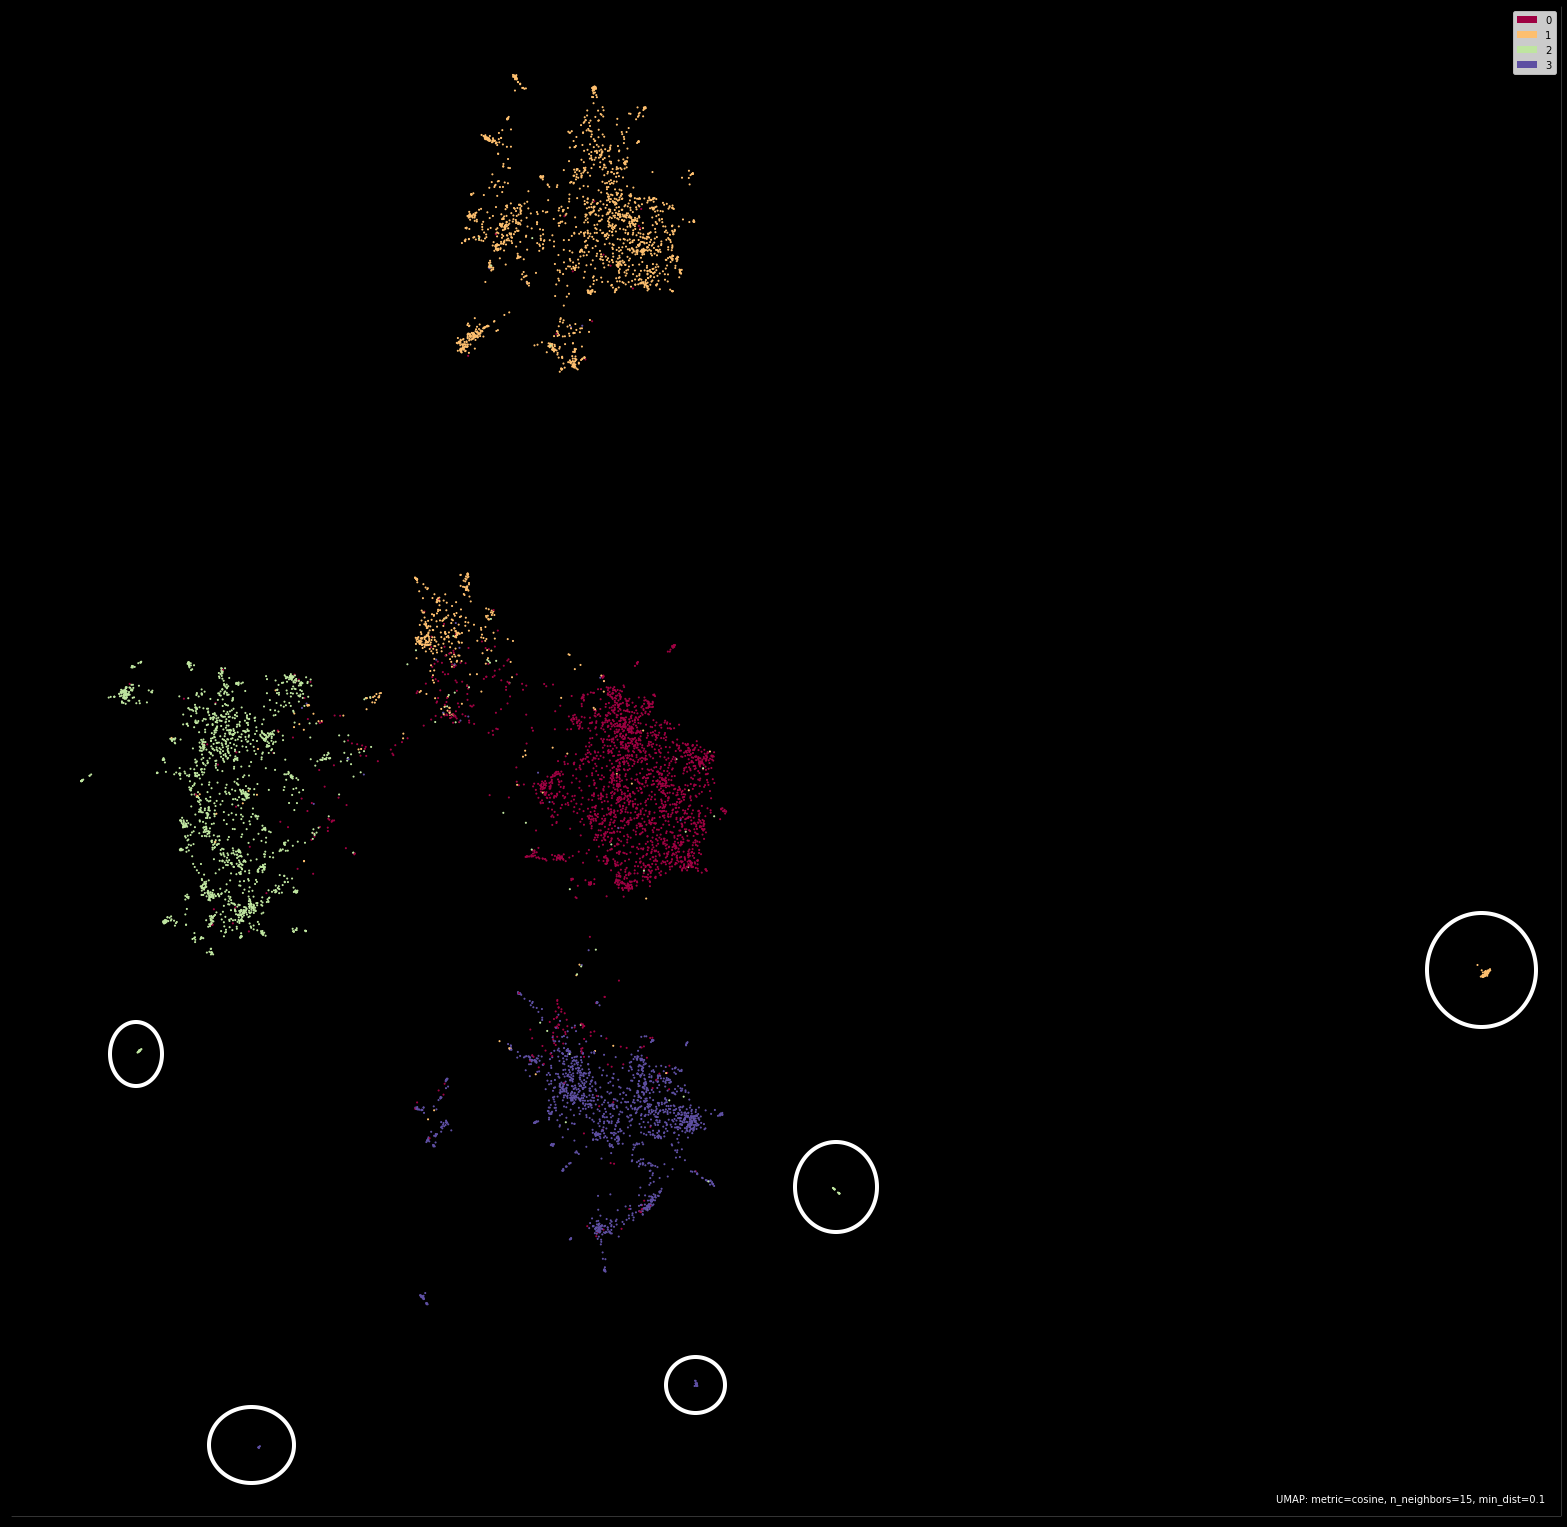
\includegraphics[width=12cm]{Figures/umap2d.png}
\centering
\caption{UMAP 2D Scatter Plot Visualization for Top2Vec}
\label{fig:umap2d}
\end{figure*}

\begin{figure*}[ht]
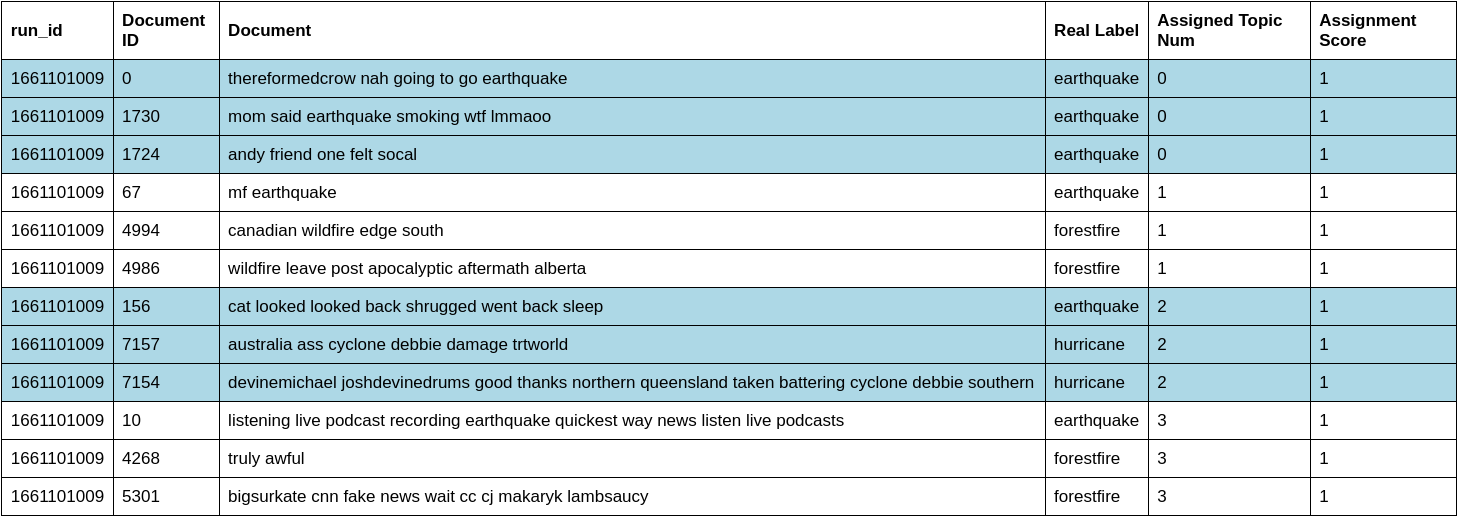
\includegraphics[width=16cm]{Figures/ldabert_get_representative_docs.png}
\centering
\caption{Representative Documents per Topic Visualization for LDA-BERT}
\label{fig:representative_docs}
\end{figure*}



\end{document}
